\usetikzlibrary{shapes,snakes}

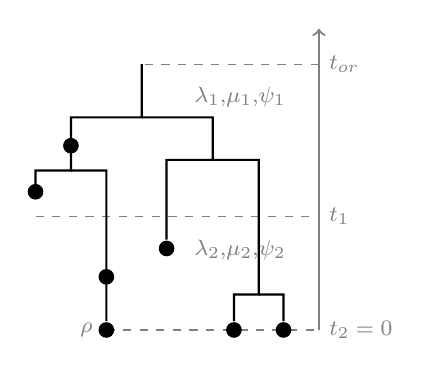
\begin{tikzpicture}[thick,scale=0.45]

\begin{scope}

\draw[ -> ,color=gray] (5, 1) -- (5, 9.5);
\draw[thin,dashed,color=gray] (5, 8.5) -- (0, 8.5);
\node[anchor=west]  at (5, 8.5) (or) {\textcolor{gray}{\footnotesize $t_{or}$}};

\draw[thin,dashed,color=gray] (-3, 4.2) -- (5, 4.2);
\node[anchor=west]  at (5, 4.2) (t1) {\textcolor{gray}{\footnotesize $t_1$}};


\draw[thin, dashed,color=gray] (-1, 1) -- (5, 1);
\node[anchor=west]  at (5, 1) (zero) {\textcolor{gray}{\footnotesize $t_2=0$}};

\node[anchor=south west]  at (1.2, 7.0) (y) {\textcolor{gray}{\footnotesize $\lambda_1$,$\mu_1$,$\psi_1$}};

\node[anchor=south west]  at (1.2, 2.7) (y) {\textcolor{gray}{\footnotesize $\lambda_2$,$\mu_2$,$\psi_2$}};

%\node[anchor=east]  at (-3.1, 4.2) (y) {\textcolor{gray}{\footnotesize $\rho_1$}};
\node[anchor=east]  at (-1.1, 1) (y) {\textcolor{gray}{\footnotesize $\rho$}};




%sampled nodes
\node[fill,circle, inner sep=2pt] at (-3, 4.9)(s2){};
\node[fill,circle, inner sep=2pt] at (0.7, 3.3)(s3){};
\node[fill,circle, inner sep=2pt] at (-2, 6.2)(s4){};
\node[fill,circle, inner sep=2pt] at (4, 1)(s5){};
\node[fill,circle, inner sep=2pt] at (-1, 1)(s8){};
\node[fill,circle, inner sep=2pt] at (-1, 2.5)(s9){};
\node[fill,circle, inner sep=2pt] at (2.6, 1)(s10){};


%branches
\draw (0, 8.5) -- (0,7) -- (-2, 7) --(-2, 5.5) --(-3, 5.5) -- (-3, 4.9) -- (s2);
\draw (-2, 5.5) -- (-1, 5.5) -- (s8); 
\draw (0,7) -- (2,7) -- (2,5.8) -- (0.7, 5.8) -- (0.7, 4.5) -- (s3); 
\draw (2, 5.8) -- (3.3, 5.8) -- (3.3, 2) -- (2.6, 2) --  (s10); 
\draw (3.3, 2) -- (4, 2) -- (s5);

\end{scope}



\end{tikzpicture}

